

\begin{figure}[t]
    \centering
    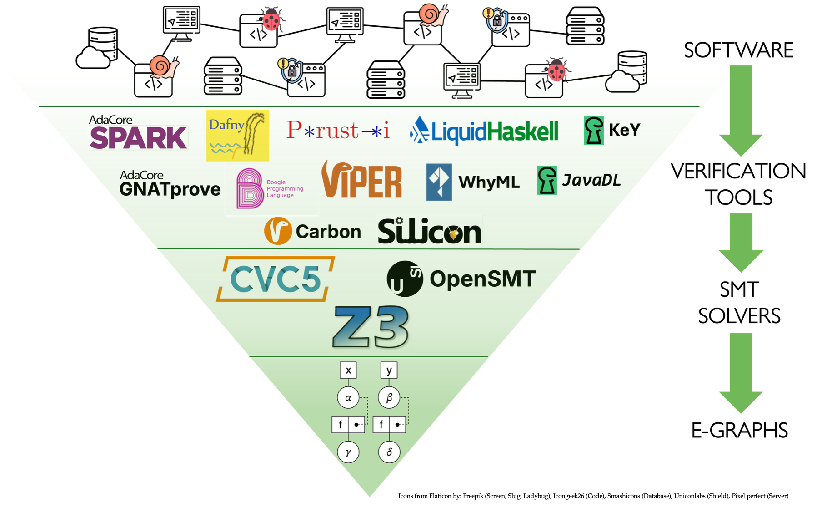
\includegraphics[width=0.7\textwidth]{figures/pyramid.pdf}
    \caption{The static verification ecosystem based on SMT solvers and e-graphs.}
\end{figure}

\textit{Software verification} is the discipline of assuring that a software system
conforms to a given specification. It is a traditional area of research in 
computer science, drawing on both \textit{software engineering} and 
\textit{programming languages}.
\textit{Dynamic verification}, such as \textit{testing} and \textit{fuzzing}, 
executes the system under selected configurations to discover deviations from 
the specification, i.e., \textit{bugs}. 
Instead, \textit{static verification}, such as \textit{model checking} and
\textit{theorem proving}, analyzes all possible system's behaviors to guarantee 
that it always satisfies the specification. Since this is rarely feasible for 
complex systems, static verification often relies on
\textit{abstractions} that approximate the system and the specification to make
the analysis tractable. In that sense, it is \textit{static} because the 
analysis is performed without executing the original system.

In this proposal, we focus on \textit{static verification} and specifically on
\textit{theorem proving} for software verification.


\paragraph{What is verification?} The process of guaranteeing that a system
satisfies a specification\dots

\paragraph{Why is it significant?} Soundness guarantees compared to testing,
formal methods for AI, \dots

\paragraph{What are the verification tools?} SMT solvers, saturation-based, eqsat-based, Lean, Coq, Isabelle, Agda, \dots

\paragraph{What are the challenges?} Scalability, usability, \dots

\paragraph{What is the contribution of this PhD proposal?} Optimizing the
verification ecosystem based on e-graphs \dots

\paragraph{What is the impact?} Proving more and faster \dots
